\documentclass[border = 0.2cm]{standalone}

% Required packages and libraries
\usepackage{tikz}
\usetikzlibrary{petri,positioning}

\begin{document}

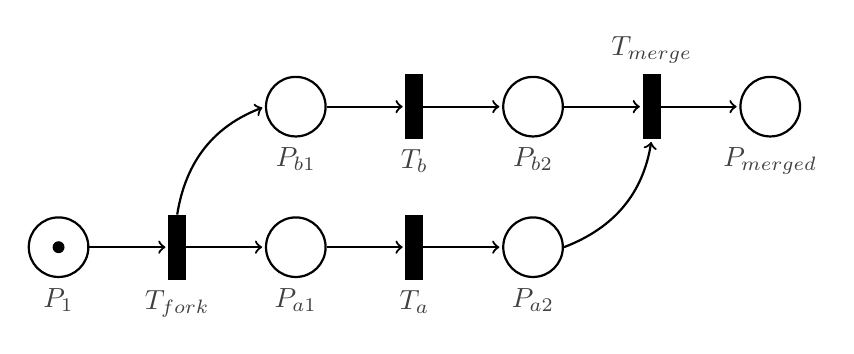
\begin{tikzpicture}[thick,
    every transition/.style={fill=black,minimum width=2mm, minimum height=8mm},
    every label/.style={black!75}]

% Place & transitions
\node[  place,
        label=below:$P_1$,
        tokens=1
    ] (place1) at (0,0) {};
\node[  transition,
        label=below:$T_{fork}$,
        right=of place1,
    ] (transfork) {};
\node[  place,
        label=below:$P_{a1}$,
        right=of transfork
    ] (place_a1) {};
\node[  place,
        label=below:$P_{b1}$,
        above=of place_a1
    ] (place_b1) {};
\node[  transition,
        label=below:$T_{b}$,
        right=of place_b1,
    ] (transb2) {};
\node[  transition,
        label=below:$T_{a}$,
        right=of place_a1,
    ] (transa2) {};
\node[  place,
        label=below:$P_{b2}$,
        right=of transb2
    ] (place_b2) {};
\node[  place,
        label=below:$P_{a2}$,
        right=of transa2
    ] (place_a2) {};
\node[  transition,
    label=above:$T_{merge}$,
    right=of place_b2
] (transmerge) {};
\node[  place,
        label=below:$P_{merged}$,
        right=of transmerge
    ] (place_merged) {};
% Arcs
\draw[thick]
    (place1) edge[post] (transfork)
    (transfork) edge[post] (place_a1)
    (place_b1) edge[post] (transb2)
    (transa2) edge[post] (place_a2)
    (place_a1) edge[post] (transa2)
    (transb2) edge[post] (place_b2)
    (place_a2.east) edge[post, bend right] (transmerge.south)
    (transmerge) edge[post] (place_merged)
    (place_b2) edge[post] (transmerge)
    (transfork.north) edge[post, bend left] (place_b1.west);
\end{tikzpicture}

\end{document}
